\subsection{Kalman GPU}
\label{sec:link2d:kalman-gpu}

The Kalman CPU approach performs the same operation over all the bubbles of all the images.
A GPU implementation was therefore evaluated, to test its potential parallelization.

\subsubsection{Algorithm}

The algorithm is the same as the previous approach, with step 2 transformed into a GPU kernel.
This kernel processes all bubbles of all images captured at the same time instant.

\subsubsection{Evaluation}

The speed is quite faster than the Kalman CPU approach, but still considerably slower than Trackpy, standing at 68 FPS.
The quality was however worse: the number of tracklets increased to about 8900, and a visual inspection found some inconsistencies (in figure~\ref{fig:linkDD:kalmangpu}, two trackelts include an unreasonable jump).

\begin{figure}
	\centerline{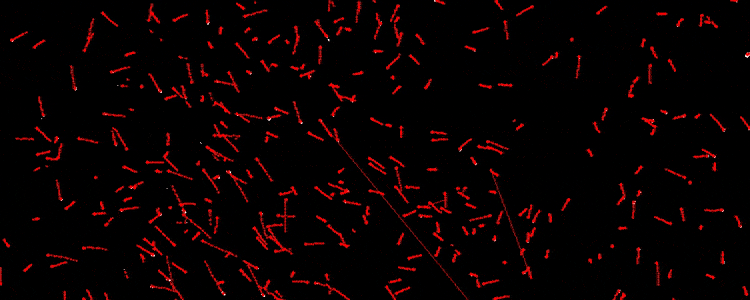
\includegraphics[width=\locateimgsize]{images/link2d/kalman_GPU.png}}
	\caption{\centering A frame from the Kalman GPU \linkDD* result, full video available at~\cite{linkDD-kalman-gpu}}
	\label{fig:linkDD:kalmangpu}
\end{figure}
